\documentclass[aspectratio=169, 11pt]{beamer}

% --- Theme & Colors ---
\usetheme{Madrid}
\usecolortheme{default}
\setbeamertemplate{navigation symbols}{}
\setbeamertemplate{footline}{%
  \hfill\insertframenumber\kern1em\vskip2pt%
}

% --- Packages ---
\usepackage{amsmath, amssymb, amsthm}
\usepackage{graphicx}
\usepackage{tikz}
\usepackage{booktabs}

% --- Blue color scheme ---
\definecolor{tseblue}{RGB}{0,70,130}
\definecolor{tselightblue}{RGB}{220,235,250}
\setbeamercolor{title}{fg=white,bg=tseblue}
\setbeamercolor{frametitle}{fg=white,bg=tseblue}
\setbeamercolor{structure}{fg=tseblue}
\setbeamercolor{block title}{fg=white,bg=tseblue}
\setbeamercolor{block body}{bg=tselightblue}
\setbeamercolor{item}{fg=tseblue}
\setbeamercolor{palette primary}{bg=tseblue,fg=white}
\setbeamercolor{palette secondary}{bg=tseblue!80,fg=white}
\setbeamercolor{palette tertiary}{bg=tseblue!60,fg=white}
\setbeamercolor{titlelike}{parent=palette primary}

% --- Title ---
\title[Armstrong \& Zhou (2022)]{Consumer Information and the Limits to Competition}
\subtitle{Armstrong \& Zhou, \textit{American Economic Review}, 2022}
\author{Jordi Torres Vallverd\'{u}}
\institute{Toulouse School of Economics}
\date{IO Theory -- MRes 2025--2026}

\begin{document}

% =============================================
% TITLE
% =============================================
\begin{frame}
\titlepage
\end{frame}

% --- Slide: Roadmap ---
\begin{frame}{Roadmap}

\begin{enumerate}
    \item \textbf{Context} -- Why information design matters for competition

    \bigskip

    \item \textbf{Model \& Main Results} -- Optimal signal structures for firms and consumers

    \bigskip

    \item \textbf{Discussion} -- Extensions, limitations, and open questions
\end{enumerate}

\end{frame}

% =============================================
% PART 1: CONTEXT / PROBLEM (~5 min)
% =============================================

% --- Slide: Why This Matters ---
\begin{frame}{Motivation}

\textbf{Platforms design the information environment consumers face}

\bigskip

\begin{itemize}
    \item Amazon, Expedia, insurance comparison sites choose:
    \begin{itemize}
        \item How much product detail to reveal
        \item Whether to offer personalized recommendations
        \item How flexibly consumers can filter and compare
    \end{itemize}

    \bigskip

    \item \textbf{Core question:} Should a platform (or regulator) make products \emph{more} or \emph{less} comparable?

    \bigskip

    \item More transparency $\Rightarrow$ better product match, but higher prices

    \item Less transparency $\Rightarrow$ fierce price competition, but potential mismatch
\end{itemize}

\end{frame}

% --- Slide: Main Idea & Tension ---
\begin{frame}{Main Idea and Key Tension}

\textbf{Central trade-off:} \; match quality \; vs.\ price competition

\bigskip

\begin{columns}[T]
\column{0.48\textwidth}
\textbf{Firm-optimal policy}
\begin{itemize}
    \item Amplifies perceived differentiation
    \item Fewer price-sensitive consumers
    \item Higher equilibrium prices
    \item \alert{No mismatch} $\Rightarrow$ max total welfare
\end{itemize}

\column{0.48\textwidth}
\textbf{Consumer-optimal policy}
\begin{itemize}
    \item Dampens perceived differentiation
    \item More price-sensitive consumers
    \item Lower equilibrium prices
    \item \alert{Some mismatch} $\Rightarrow$ welfare loss
\end{itemize}
\end{columns}


\end{frame}

% --- Slide: Literature ---
\begin{frame}{Contribution to the Literature}

\textbf{Information design meets oligopoly pricing}

\bigskip

\begin{itemize}
    \item \textbf{Monopoly information design} (Roesler \& Szentes, 2017)
    \begin{itemize}
        \item[$\rightarrow$] Extends to duopoly; competition changes the problem fundamentally
    \end{itemize}

    \medskip

    \item \textbf{Bayesian persuasion} (Kamenica \& Gentzkow, 2011)
    \begin{itemize}
        \item[$\rightarrow$] Applies persuasion framework to competitive pricing
    \end{itemize}

    \medskip

    \item \textbf{Competitive disclosure} (Anderson \& Renault, 2006; Johnson \& Myatt, 2006)
    \begin{itemize}
        \item[$\rightarrow$] Goes beyond ``truth or noise'' to general signal structures
    \end{itemize}

    \medskip

    \item \textbf{Centralized vs.\ decentralized design} (Ivanov, 2013; Hwang et al., 2019)
    \begin{itemize}
        \item[$\rightarrow$] Centralized design allows \emph{relative} signals (e.g., ``top product'')
    \end{itemize}
\end{itemize}

\end{frame}

% =============================================
% PART 2: MODEL (~5 min)
% =============================================

% --- Slide: Setup ---
\begin{frame}{Model Setup}

\begin{itemize}
    \item Two firms ($i = 1,2$) supply differentiated products at zero cost

    \medskip

    \item Consumer values product $i$ at $v_i \geq 0$; prior on $(v_1, v_2)$ is symmetric

    \medskip

    \item Only the \textbf{relative preference} matters: $x \equiv v_1 - v_2$
    \begin{itemize}
        \item Prior CDF $F(x)$ symmetric around 0, support $[-1,1]$
    \end{itemize}

    \medskip

    \item Consumer observes a \textbf{private signal} $s$ before purchase
    \begin{itemize}
        \item Signal structure $\{\sigma(s|x), S\}$ is public and chosen \emph{before} firms set prices
    \end{itemize}

    \medskip

    \item After signal $s$, consumer updates to \textbf{posterior} $G(x) \equiv$ CDF of $E_{F_s}[x]$

    \medskip

    \item Firms observe $G$ but not $s$; set prices simultaneously (Bertrand--Nash)

    \medskip

    \item Consumer buys from firm 1 if $E[x \mid s] > p_1 - p_2$
\end{itemize}

\end{frame}

% --- Slide: Key Constraint ---
\begin{frame}{Key Constraint: Mean-Preserving Contraction}

\textbf{Bayesian consistency:} any posterior $G$ must be a \textbf{mean-preserving contraction} (MPC) of the prior $F$:

$$\int_{-1}^{x} G(\tilde{x})\, d\tilde{x} \;\leq\; \int_{-1}^{x} F(\tilde{x})\, d\tilde{x} \qquad \text{for all } x \in [-1,1]$$

\bigskip

\begin{itemize}
    \item Signals can reshuffle beliefs inward, but cannot create information from nothing

    \bigskip

    \item Any $G$ satisfying MPC can be induced by some signal structure

    \bigskip

    \item $\Rightarrow$ Instead of optimizing over signals, we optimize directly over the posterior $G$
\end{itemize}

\end{frame}

% --- Slide: Lemma 1 ---
\begin{frame}{Bounds on Equilibrium Posteriors}

\begin{block}{Lemma 1}
$G$ implements symmetric price $p$ in pure-strategy equilibrium \textbf{iff}
$$L_{p}(x) \;\leq\; G(x) \;\leq\; U_{p}(x) \qquad \forall\, x \in [-1,1]$$
\end{block}

\medskip

\textbf{Upper bound} (from firm 2's no-deviation condition):

\begin{itemize}
    \item Firm 2 deviates to $p_2'$. Profit from deviation: $p_2' \cdot G(p_1 - p_2')$

    \medskip

    \item No deviation is profitable iff $\;p_2'\, G(p_1 - p_2') \leq \pi_2 = p/2\;$ for all $p_2'$

    \medskip

    \item Substituting $x = p - p_2'$ and rearranging:
    $$G(x) \;\leq\; \frac{p}{2(p - x)} \;\equiv\; U_p(x) \qquad \text{for } x < \tfrac{1}{2}p$$
\end{itemize}

\medskip

\textbf{Lower bound} $L_p(x) = 1 - \frac{p}{2(p+x)}$: symmetric argument for firm 1

\medskip

\small
$L_p$ and $U_p$ are mirror images: $L_p(x) = 1 - U_p(-x)$

\end{frame}

% --- Slide: Symmetry Result ---
\begin{frame}{Symmetric Signals Dominate}

\begin{block}{Lemma 2}
Relative to any \emph{asymmetric} posterior (one that treats firms differently):
\begin{enumerate}
    \item[(i)] There exists a \textbf{symmetric} posterior with \textbf{higher profit for each firm}
    \item[(ii)] There exists a \textbf{symmetric} posterior with \textbf{higher consumer surplus}
\end{enumerate}
\end{block}

\bigskip

\textbf{Intuition:}
\begin{itemize}
    \item Biased signals favor one firm $\Rightarrow$ the other undercuts aggressively
    \item The resulting price war hurts \emph{both} firms --- even the favored one
    \item For consumers: asymmetry causes mismatch + price dispersion
\end{itemize}

\bigskip

$\Rightarrow$ \textbf{We can restrict attention to symmetric signal structures}

\end{frame}

% --- Slide: Proposition 1 - Intuition ---
\begin{frame}{Firm-Optimal Signal: Intuition}

\textbf{Goal:} find the highest sustainable price $p$

\bigskip

\begin{enumerate}
    \item Higher $p$ $\Rightarrow$ the feasibility corridor $[L_p, U_p]$ becomes flatter

    \bigskip

    \item To fit inside a flat corridor \emph{and} satisfy MPC, $G$ is squeezed against the \textbf{lower bound} $L_p$ on $[-1,0]$

    \bigskip

    \item $G = L_p$ $\Rightarrow$ \textbf{few near-indifferent consumers} (U-shaped density)
    \begin{itemize}
        \item Neither firm can profitably undercut $\Rightarrow$ high price is sustainable
        \item Everyone has strong preferences $\Rightarrow$ buys preferred product $\Rightarrow$ \textbf{no mismatch}
    \end{itemize}
\end{enumerate}

\bigskip

Push $p$ until MPC binds $\Rightarrow$ \textbf{the maximum feasible price}

\end{frame}

% --- Slide: Proposition 1 - Result ---
\begin{frame}{Firm-Optimal Signal: Result}

\begin{block}{Proposition 1}
The firm-optimal signal induces the symmetric equilibrium price:
$$p^* \;=\; \frac{2\delta}{1 - \log 2} \;\approx\; 6.5\,\delta$$
where $\delta \equiv E_F[\max\{x,0\}]$ measures how differentiated products are.\\
Implemented by $G(x) = L_{p^*}(x)$ for $x < 0$.
\end{block}

\bigskip

\begin{itemize}
    \item Higher $\delta$ (more differentiation) $\Rightarrow$ higher optimal price

    \bigskip

    \item \textbf{No mismatch} $\Rightarrow$ total welfare is maximized ($= \mu + \delta$)

    \bigskip

    \item Profit $\geq 63\%$ higher than under full disclosure
\end{itemize}

\end{frame}

% --- Slide: Figure - Firm-Optimal Posterior ---
\begin{frame}{Firm-Optimal Posterior (Uniform Prior)}

\begin{center}
    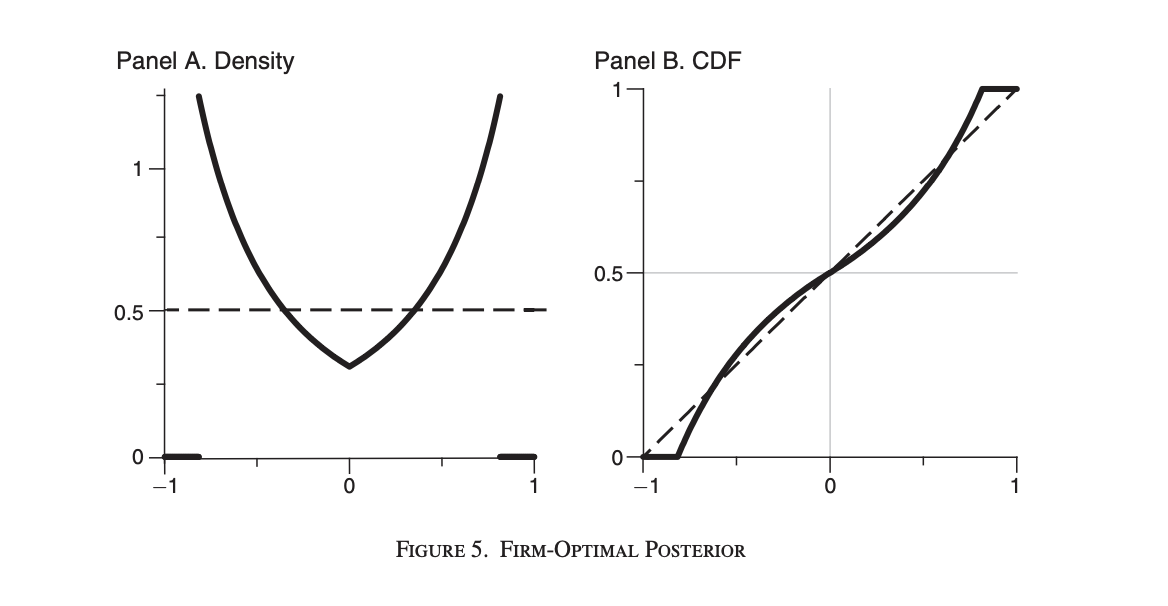
\includegraphics[width=0.75\textwidth]{table1.png}
\end{center}

\smallskip

\small
Dashed = uniform prior. \; Solid = firm-optimal posterior $G = L_{p^*}$.\\[3pt]
U-shaped density: mass at extremes, few indifferent consumers $\Rightarrow$ high price.

\end{frame}

% --- Slide: Proposition 2 - Intuition ---
\begin{frame}{Consumer-Optimal Signal: Intuition}

\textbf{Goal:} maximize consumer surplus $= $ match value $-$ price

\bigskip

\begin{enumerate}
    \item Consumers want fierce price competition $\Rightarrow$ need \textbf{many near-indifferent consumers}

    \bigskip

    \item This means pushing $G$ against the \textbf{upper bound} $U_p$ on $[-1,0]$
    \begin{itemize}
        \item Density peaked near $x = 0$ $\Rightarrow$ firms terrified of losing swing consumers
        \item Each firm undercuts aggressively $\Rightarrow$ very low price
    \end{itemize}

    \bigskip

    \item \textbf{Cost:} some near-indifferent consumers buy the wrong product (mismatch)

    \bigskip

    \item But the \textbf{price drop more than compensates} for match quality loss
\end{enumerate}

\end{frame}

% --- Slide: Proposition 2 - Result ---
\begin{frame}{Consumer-Optimal Signal: Result}

\begin{block}{Proposition 2}
The consumer-optimal signal induces price:
$$p^{**} \;=\; \frac{-\gamma}{1 - \gamma}\, F^{-1}\!\Big(\frac{\gamma}{2}\Big), \qquad \gamma \approx 0.05$$
Implemented by: \; $G(x) \;=\; \min\big\{F(x),\; U_{p^{**}}(x)\big\}$ for $x < 0$
\end{block}

\bigskip

\begin{itemize}
    \item \textbf{Mismatch occurs} --- total welfare $< \mu + \delta$

    \bigskip

    \item Price effect dominates $\Rightarrow$ higher consumer surplus than full disclosure

    \bigskip

    \item $G = \min\{F, U_p\}$: posterior follows the prior until it hits the upper bound, then rides along it --- blurring only weak preferences
\end{itemize}

\end{frame}

% --- Slide: Figure - Consumer-Optimal Posterior ---
\begin{frame}{Consumer-Optimal Posterior (Uniform Prior)}

\begin{center}
    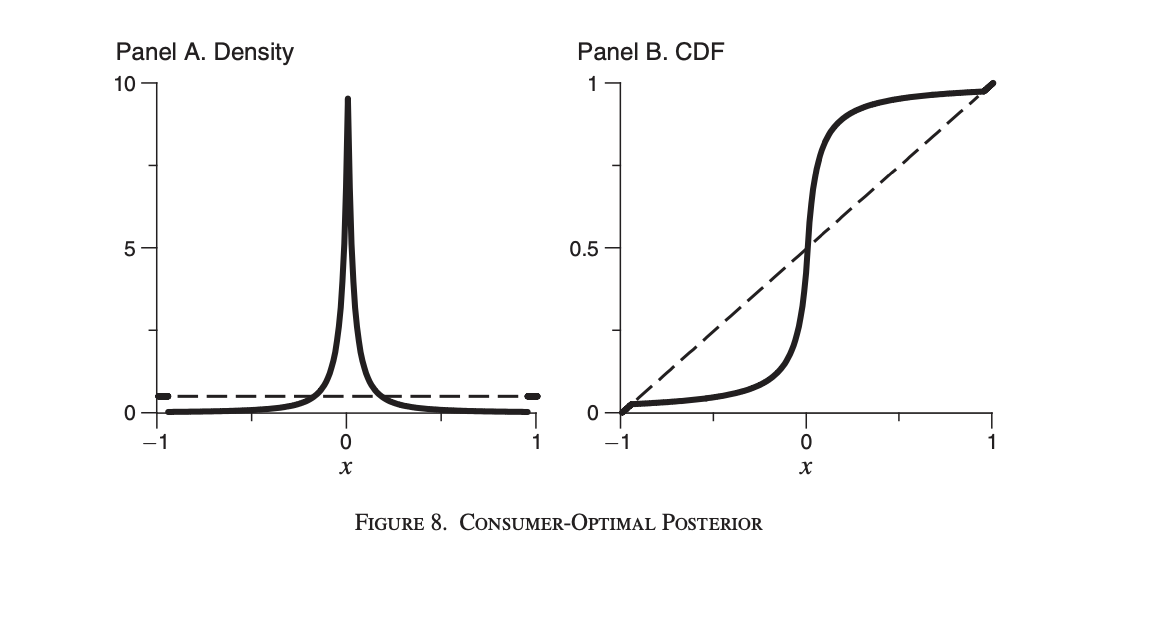
\includegraphics[width=0.70\textwidth]{table2.png}
\end{center}

\smallskip

\small
Dashed = uniform prior. \; Solid = consumer-optimal posterior.\\[3pt]
Spike near $x = 0$: many nearly indifferent consumers $\Rightarrow$ very low price.

\end{frame}

% =============================================
% PART 3: DISCUSSION (~5 min)
% =============================================

% --- Slide: Proposition 3 ---
\begin{frame}{The Limits to Competition}

\begin{block}{Proposition 3}
Any profit $p \in [0, p^*]$ is feasible. For a given profit level $p$:
\begin{itemize}
    \item \textbf{Min CS:} \; $\mu - \tfrac{1}{2}(1 + \log 2)\,p$ \quad (posterior $= L_p$)
    \item \textbf{Max CS:} \; $\mu + \delta - p$ when $p \geq p_F$; \; concave frontier when $p < p_F$
\end{itemize}
\end{block}

\medskip

\textbf{Key implication:} competition makes it \textbf{impossible} to have both low profit \emph{and} low CS simultaneously

\begin{itemize}
    \item Full disclosure optimal \emph{only} for unweighted total welfare
    \item Ramsey problem picks a point on the feasible frontier
    \item Contrast with monopoly (Roesler \& Szentes, 2017): there low profit \emph{and} low CS is feasible
\end{itemize}

\end{frame}

% --- Slide: Figure - Feasible Frontier ---
\begin{frame}{Feasible Combinations of Profit and Consumer Surplus}

\begin{center}
    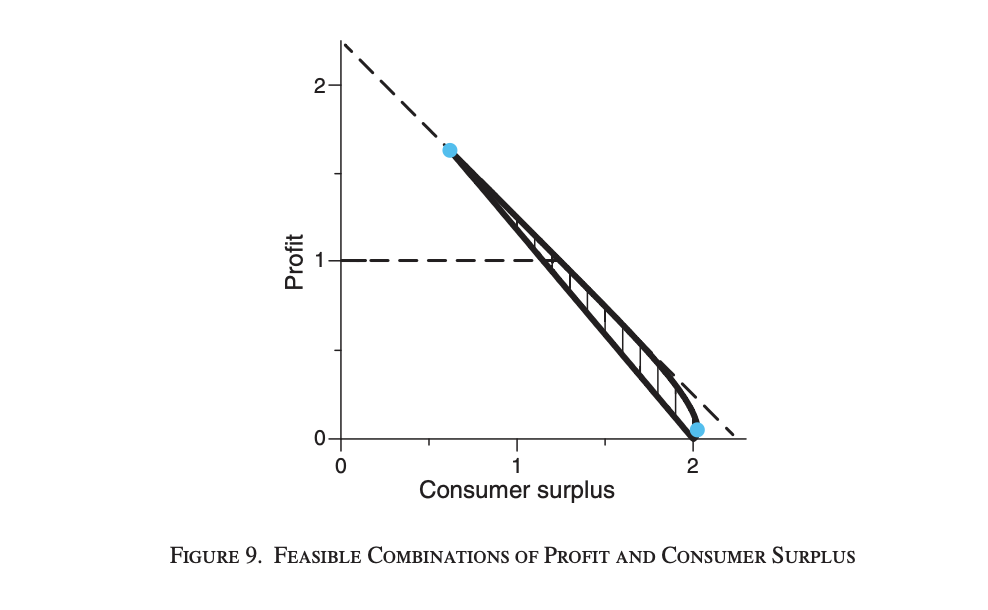
\includegraphics[width=0.6\textwidth]{table3.png}
\end{center}

\smallskip

\small
Shaded area = feasible (profit, CS) pairs. Upper-left dot = firm-optimal; lower-right dot = consumer-optimal. Dashed line = max total welfare $\mu + \delta$.\\[3pt]
Due to competition, the feasible set cannot reach the origin.

\end{frame}

% --- Slide: Summary of Results ---
\begin{frame}{Summary of Results}

\renewcommand{\arraystretch}{1.4}
\begin{center}
\begin{tabular}{l c c}
\toprule
 & \textbf{Firm-optimal} & \textbf{Consumer-optimal} \\
\midrule
Price & $p^* = \frac{2\delta}{1-\log 2} \approx 6.5\delta$ & $p^{**} \approx 0.05\, p_F$ \\[4pt]
Posterior & $G = L_{p^*}$ (lower bound) & $G = \min\{F, U_{p^{**}}\}$ \\[4pt]
Mismatch? & \textbf{No} & \textbf{Yes} \\[4pt]
Total welfare & Maximized ($\mu + \delta$) & Not maximized \\[4pt]
Symmetric? & Yes & Yes \\
\bottomrule
\end{tabular}
\end{center}

\bigskip

\begin{itemize}
    \item More information $\neq$ more competition
    \item Biased recommendations never help either side (Lemma 2)
    \item Competition prevents simultaneously low profit \emph{and} low CS (Prop.\ 3)
\end{itemize}

\end{frame}

% --- Slide: Extensions ---
\begin{frame}{Extensions}

\textbf{1. Mixed-strategy equilibria}
\begin{itemize}
    \item Allowing mixed strategies improves CS by at most 1.6\%
    \item Pure-strategy restriction is essentially without loss
\end{itemize}

\bigskip

\textbf{2. More than two firms}
\begin{itemize}
    \item ``Top product'' signal: can achieve first-best profit for firms
    \item ``Top two'' signal: induces Bertrand $\Rightarrow$ $p = 0$, best for consumers
    \item As $n \to \infty$: trade-off between price and match quality vanishes
\end{itemize}

\end{frame}

% --- Slide: Discussion & Open Questions ---
\begin{frame}{Discussion and Open Questions}

\begin{itemize}
    \item Scalar heterogeneity ($x = v_1 - v_2$): multi-dimensional preferences are harder

    \bigskip

    \item Symmetric firms: what if one firm is known to be better (vertical differentiation)?

    \bigskip

    \item Information designer as strategic agent (platform with own objective)?

    \bigskip

    \item Endogenous product design: firms may adjust products in response to signals
    \item \textbf{Find extensions that are easily implemented.}
    \end{itemize}

\end{frame}

\end{document}
